% Options for packages loaded elsewhere
% Options for packages loaded elsewhere
\PassOptionsToPackage{unicode}{hyperref}
\PassOptionsToPackage{hyphens}{url}
\PassOptionsToPackage{dvipsnames,svgnames,x11names}{xcolor}
%
\documentclass[
]{article}
\usepackage{xcolor}
\usepackage[left=1in,right=1in,top=1in,bottom=1in]{geometry}
\usepackage{amsmath,amssymb}
\setcounter{secnumdepth}{-\maxdimen} % remove section numbering
\usepackage{iftex}
\ifPDFTeX
  \usepackage[T1]{fontenc}
  \usepackage[utf8]{inputenc}
  \usepackage{textcomp} % provide euro and other symbols
\else % if luatex or xetex
  \usepackage{unicode-math} % this also loads fontspec
  \defaultfontfeatures{Scale=MatchLowercase}
  \defaultfontfeatures[\rmfamily]{Ligatures=TeX,Scale=1}
\fi
\usepackage{lmodern}
\ifPDFTeX\else
  % xetex/luatex font selection
  \setmainfont[]{Latin Modern Roman}
\fi
% Use upquote if available, for straight quotes in verbatim environments
\IfFileExists{upquote.sty}{\usepackage{upquote}}{}
\IfFileExists{microtype.sty}{% use microtype if available
  \usepackage[]{microtype}
  \UseMicrotypeSet[protrusion]{basicmath} % disable protrusion for tt fonts
}{}
\makeatletter
\@ifundefined{KOMAClassName}{% if non-KOMA class
  \IfFileExists{parskip.sty}{%
    \usepackage{parskip}
  }{% else
    \setlength{\parindent}{0pt}
    \setlength{\parskip}{6pt plus 2pt minus 1pt}}
}{% if KOMA class
  \KOMAoptions{parskip=half}}
\makeatother
% Make \paragraph and \subparagraph free-standing
\makeatletter
\ifx\paragraph\undefined\else
  \let\oldparagraph\paragraph
  \renewcommand{\paragraph}{
    \@ifstar
      \xxxParagraphStar
      \xxxParagraphNoStar
  }
  \newcommand{\xxxParagraphStar}[1]{\oldparagraph*{#1}\mbox{}}
  \newcommand{\xxxParagraphNoStar}[1]{\oldparagraph{#1}\mbox{}}
\fi
\ifx\subparagraph\undefined\else
  \let\oldsubparagraph\subparagraph
  \renewcommand{\subparagraph}{
    \@ifstar
      \xxxSubParagraphStar
      \xxxSubParagraphNoStar
  }
  \newcommand{\xxxSubParagraphStar}[1]{\oldsubparagraph*{#1}\mbox{}}
  \newcommand{\xxxSubParagraphNoStar}[1]{\oldsubparagraph{#1}\mbox{}}
\fi
\makeatother


\usepackage{longtable,booktabs,array}
\newcounter{none} % for unnumbered tables
\usepackage{calc} % for calculating minipage widths
% Correct order of tables after \paragraph or \subparagraph
\usepackage{etoolbox}
\makeatletter
\patchcmd\longtable{\par}{\if@noskipsec\mbox{}\fi\par}{}{}
\makeatother
% Allow footnotes in longtable head/foot
\IfFileExists{footnotehyper.sty}{\usepackage{footnotehyper}}{\usepackage{footnote}}
\makesavenoteenv{longtable}
\usepackage{graphicx}
\makeatletter
\newsavebox\pandoc@box
\newcommand*\pandocbounded[1]{% scales image to fit in text height/width
  \sbox\pandoc@box{#1}%
  \Gscale@div\@tempa{\textheight}{\dimexpr\ht\pandoc@box+\dp\pandoc@box\relax}%
  \Gscale@div\@tempb{\linewidth}{\wd\pandoc@box}%
  \ifdim\@tempb\p@<\@tempa\p@\let\@tempa\@tempb\fi% select the smaller of both
  \ifdim\@tempa\p@<\p@\scalebox{\@tempa}{\usebox\pandoc@box}%
  \else\usebox{\pandoc@box}%
  \fi%
}
% Set default figure placement to htbp
\def\fps@figure{htbp}
\makeatother





\setlength{\emergencystretch}{3em} % prevent overfull lines

\providecommand{\tightlist}{%
  \setlength{\itemsep}{0pt}\setlength{\parskip}{0pt}}



 


\setlength{\footskip}{65pt}
\usepackage[font=scriptsize]{caption}
\usepackage[noblocks]{authblk}
\renewcommand*{\Authsep}{, }
\renewcommand*{\Authand}{, }
\renewcommand*{\Authands}{, }
\renewcommand\Affilfont{\small}
\renewcommand{\thefootnote}{\alph{footnote}}
\usepackage{etoolbox}
\AtEndEnvironment{abstract}{\noindent\textbf{Keywords:} \KeywordList \par}
\makeatletter
\@ifpackageloaded{caption}{}{\usepackage{caption}}
\AtBeginDocument{%
\ifdefined\contentsname
  \renewcommand*\contentsname{Table of contents}
\else
  \newcommand\contentsname{Table of contents}
\fi
\ifdefined\listfigurename
  \renewcommand*\listfigurename{List of Figures}
\else
  \newcommand\listfigurename{List of Figures}
\fi
\ifdefined\listtablename
  \renewcommand*\listtablename{List of Tables}
\else
  \newcommand\listtablename{List of Tables}
\fi
\ifdefined\figurename
  \renewcommand*\figurename{Figure}
\else
  \newcommand\figurename{Figure}
\fi
\ifdefined\tablename
  \renewcommand*\tablename{Table}
\else
  \newcommand\tablename{Table}
\fi
}
\@ifpackageloaded{float}{}{\usepackage{float}}
\floatstyle{ruled}
\@ifundefined{c@chapter}{\newfloat{codelisting}{h}{lop}}{\newfloat{codelisting}{h}{lop}[chapter]}
\floatname{codelisting}{Listing}
\newcommand*\listoflistings{\listof{codelisting}{List of Listings}}
\makeatother
\makeatletter
\makeatother
\makeatletter
\@ifpackageloaded{caption}{}{\usepackage{caption}}
\@ifpackageloaded{subcaption}{}{\usepackage{subcaption}}
\makeatother
\usepackage{bookmark}
\IfFileExists{xurl.sty}{\usepackage{xurl}}{} % add URL line breaks if available
\urlstyle{same}
\hypersetup{
  pdftitle={Little evidence for meaningful intervention effect heterogeneity in resistance training: Evidence from causal inference and meta-analytic variance comparisons},
  pdfauthor={James Steele},
  pdfkeywords={resistance training, heterogeneity, individual
response, causal inference, meta-analysis},
  colorlinks=true,
  linkcolor={blue},
  filecolor={Maroon},
  citecolor={Blue},
  urlcolor={Blue},
  pdfcreator={LaTeX via pandoc}}


\title{Little evidence for meaningful intervention effect heterogeneity
in resistance training: Evidence from causal inference and meta-analytic
variance comparisons\thanks{Preprint, please cite as: Steele, J. (2026).
Little evidence for meaningful intervention effect heterogeneity in
resistance training: Evidence from causal inference and meta-analytic
variance comparisons. sportrxiv DOI:
\url{https://doi.org/10.51224/SportRxiv.783}. Address for
correspondence: james@steele-research.com}}


\author[1,2,3]{James Steele}

\affil[1]{Steele Research Limited, Eastleigh, Hampshire, UK}
\affil[2]{MacroFactor, Stronger by Science Technologies LLC, Raleigh,
North Carolina, USA}
\affil[3]{School of Health and Biomedical Sciences, Royal Melbourne
Institute of Technology, Melbourne, VIC, Australia}

% Store the keywords (expanded by Pandoc here)
\def\KeywordList{resistance training, heterogeneity, individual
response, causal inference, meta-analysis}

\date{July 10, 2026}
\begin{document}
\maketitle
\begin{abstract}
Resistance training studies consistently demonstrate substantial
variation in observed outcomes between participants. This variation is
commonly interpreted as evidence that individuals differ meaningfully in
their responses to training interventions. However, observed variation
in outcomes does not necessarily imply heterogeneity in the underlying
causal effects of an intervention. Rather, observed outcomes reflect
multiple sources of variation, including between-participant
differences, within-participant variability, measurement error, and
potentially true intervention effect heterogeneity. Within the potential
outcomes framework, heterogeneity of intervention effects is
fundamentally a question about the variance of causal effects. Although
directly estimating this variance generally requires specialised study
designs such as randomised replicated crossover trials, traditional
randomised controlled trials (RCTs) comparing an intervention against an
inert control can provide indirect evidence regarding intervention
effect heterogeneity through comparisons of outcome variances. Here, I
outline the causal framework underpinning variance comparisons, discuss
the assumptions required for causal interpretation, and demonstrate how
meta-analytic models can synthesise evidence across studies to compare
variances while accounting for the ubiquitous relationship between means
and variances. Applying these methods to a large meta-analytic dataset
of RCTs of resistance training interventions reveals little evidence
that interventions meaningfully increase outcome variability beyond that
expected from the increase in mean outcomes themselves. Although
conclusions necessarily depend upon assumptions regarding the
correlation between potential outcomes, these assumptions appear
empirically reasonable for resistance training studies in healthy
participants. Taken together, current evidence provides little support
for the existence of substantial intervention effect heterogeneity in
resistance training adaptations.
\end{abstract}


\section{Introduction}\label{introduction}

Variation in responses to resistance training has become a topic of
considerable interest within sport and exercise science. Large
differences are routinely observed between participants following
apparently identical training programmes for the outcomes captured, and
these differences are frequently interpreted as evidence that
individuals differ meaningfully in their responsiveness to training.
Such interpretations underpin discussions of ``responders'' and
``non-responders'', personalised exercise prescription, and the search
for biological determinants of intervention responsiveness. However,
most people working on this topic confuse the observed variation in
\emph{outcomes} with there necessarily being heterogeneity in the
\emph{underlying effect of an intervention}. This typically has involved
merely considering the distribution of outcomes observed in the
intervention arms of trials which is insufficient for determining
whether such variance is due to the effects of the intervention
themselves varying between individuals. But, careful consideration of
the underlying causal structure of the question of intervention effect
heterogeneity allows us to better evaluate whether there is or is not
evidence suggesting it is present.

Partitioning of variance components of observed outcomes such that we
can draw inferences regarding the presence (or not) of heterogeneity in
the underlying causal effect of treatment is incredibly difficult.
Typically, study designs such as those used by Robinson et al.~(2025)
(i.e., randomised replicated crossovers) are required. But, in the
context of a traditional randomised controlled trial (RCT) where the
control can be reasonably assumed to be inert (i.e., has no effect
itself), such as a non-training control in studies of healthy
untrained\footnote{Untrained participants given in a trained population
  we might expect \emph{a priori} that a detraining effect may occur
  after cessation of their training. In the case of trained
  participants, as others have argued (\textbf{ADD REF}), continuation
  of existing training may be a better control condition and indeed
  especially so when participants are already sufficiently trained
  (i.e., having trained consistently and using known effective
  interventions for at least one full year \textbf{ADD REFS}) such that
  they are no longer experiencing meaningful intervention effects
  anyway.} participants, we can obtain some insight into whether
interindividual heterogeneity in intervention effects may be present.

\begin{figure}

\begin{minipage}[t]{0.50\linewidth}

\raisebox{-\height}{

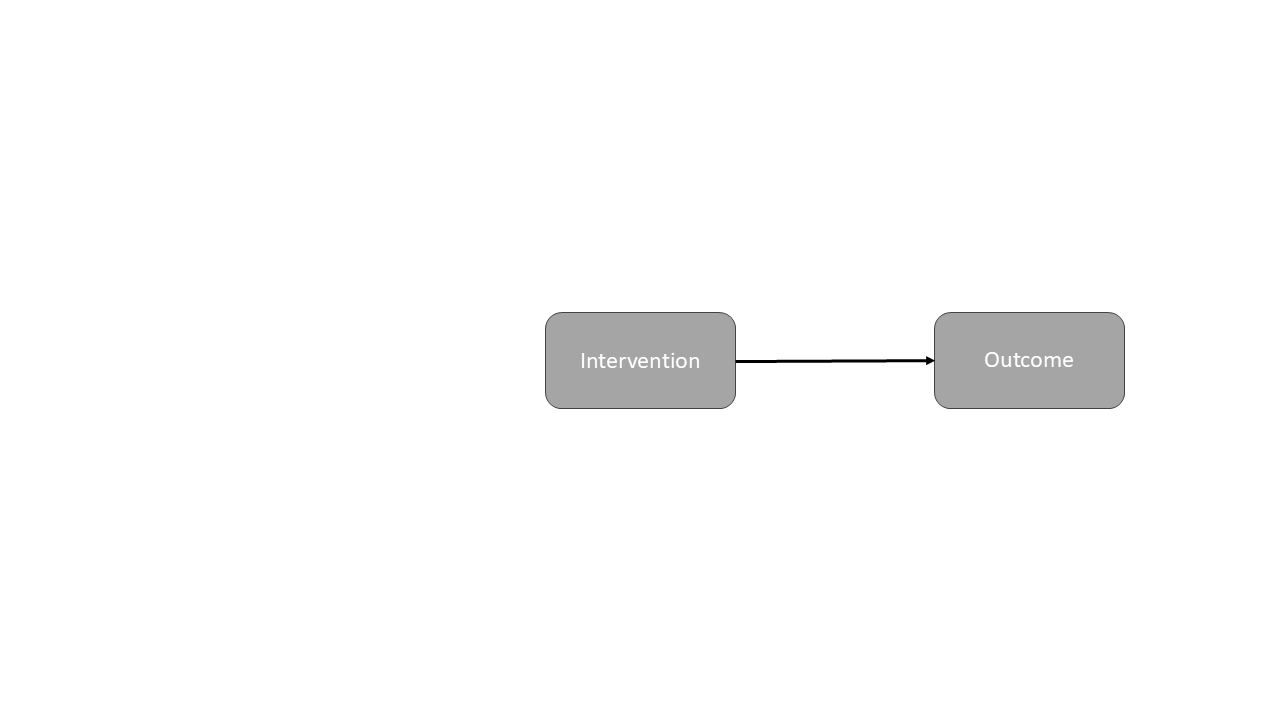
\includegraphics[width=\linewidth,height=8cm,keepaspectratio,alt={Intervention}]{images/Slide4.png}

}

\subcaption{\label{}Intervention}
\end{minipage}%
%
\begin{minipage}[t]{0.50\linewidth}

\raisebox{-\height}{

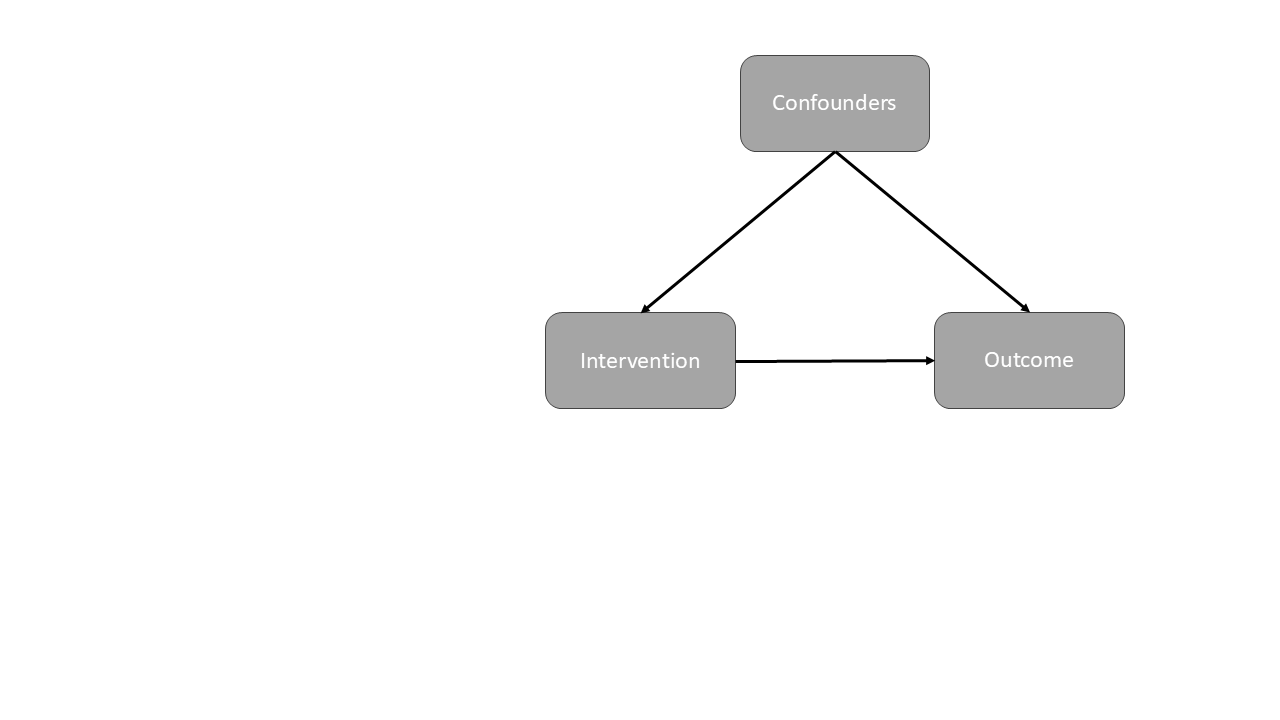
\includegraphics[width=\linewidth,height=8cm,keepaspectratio,alt={Confounders}]{images/Slide5.png}

}

\subcaption{\label{}Confounders}
\end{minipage}%
\newline
\begin{minipage}[t]{0.50\linewidth}

\raisebox{-\height}{

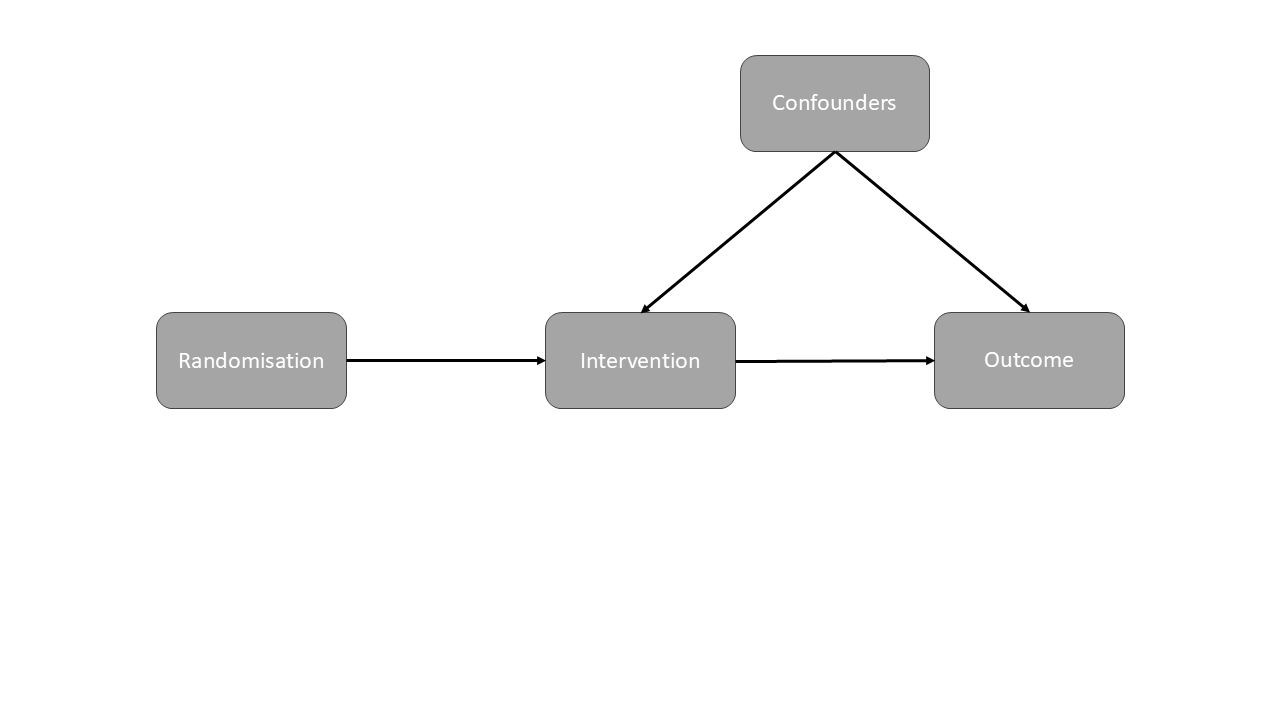
\includegraphics[width=\linewidth,height=8cm,keepaspectratio,alt={Randomisation}]{images/Slide7.png}

}

\subcaption{\label{}Randomisation}
\end{minipage}%
%
\begin{minipage}[t]{0.50\linewidth}

\raisebox{-\height}{

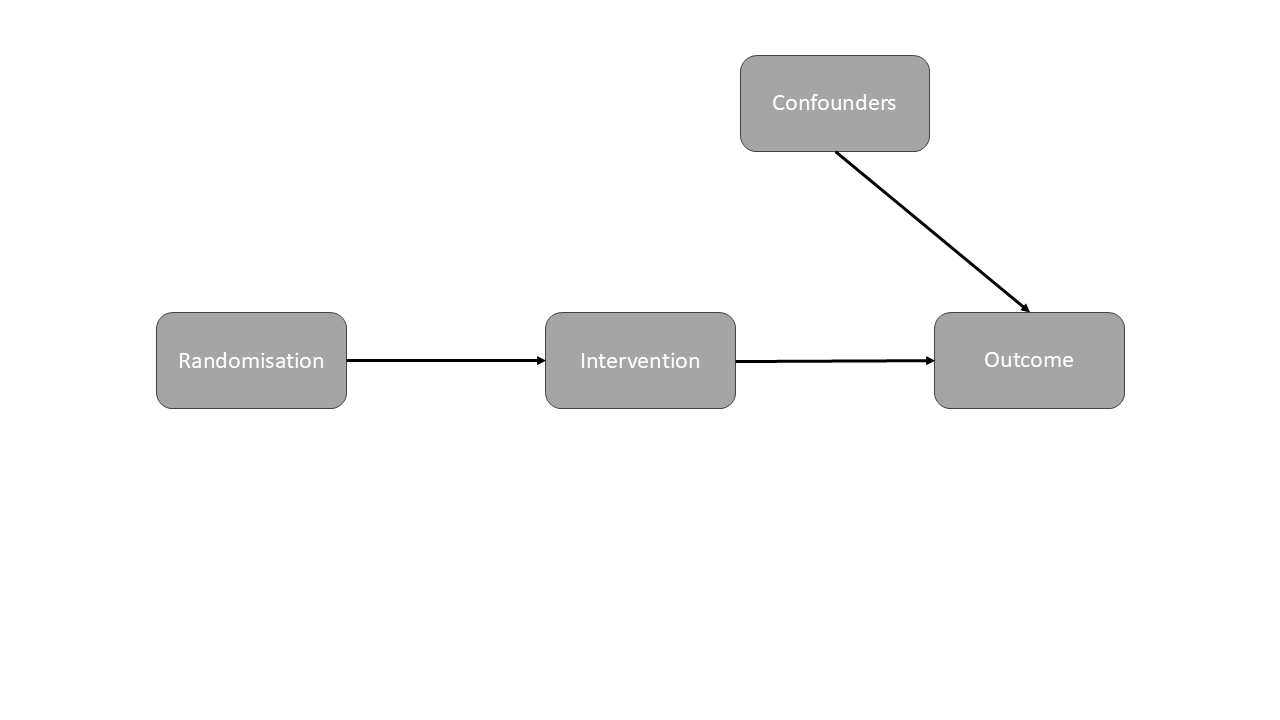
\includegraphics[width=\linewidth,height=8cm,keepaspectratio,alt={No back-door pathway}]{images/Slide8.png}

}

\subcaption{\label{}No back-door pathway}
\end{minipage}%

\caption{\label{fig-rct-logic}Logic of randomised controlled trial
design shown via directed acyclic graphs for estimating average
intervention effects. In (a) we want to estimate the causal effect of an
intervention upon some outcome, but as in (b) there are often
confounders that influence whether the intervention is participated in
and the outcome.As such, we randomise participants to receive the
intervention (c) and now this means that we can obtain an unbiased
estimate of the intervention effect because the only thing that causes
participation in the intervention is randomisation (d) i.e., there is no
``back-door'' causal pathway between the outcome and the intervention.}

\end{figure}%

The logic of the RCT design (Figure~\ref{fig-rct-logic}) allows us to
obtain an unbiased estimate of the clearly defined estimand that is the
average intervention effect (Equation~\ref{eq-ate-estimand}) through
comparison of the marginal distributions of outcomes between the
conditions e.g., intervention vs control
(Equation~\ref{eq-ate-estimate}).

\begin{equation}\protect\phantomsection\label{eq-ate-estimand}{
\begin{gathered}
\text{Estimand: Average intervention effect} \\
D = Y_{\mathrm{Int}} - Y_{\mathrm{Con}}
\end{gathered}
}\end{equation}

\begin{equation}\protect\phantomsection\label{eq-ate-estimate}{
\begin{gathered}
\text{Estimate: marginal distributions of outcomes between the conditions} \\
\overline{D}=\overline{Y_{Int}}-\overline{Y_{Con}} 
\end{gathered}
}\end{equation}

This estimand, along with its standard deviation (Equation~\ref{eq-sd}),
are well defined under the potential outcomes framework (Caldwell et
al., 2025).

\begin{equation}\protect\phantomsection\label{eq-sd}{
\begin{gathered}
\text{Standard deviation of intervention effect} \\
\sigma_{D}^2=\sigma_{Int}^2+\sigma_{Con}^2-2\sigma_{Int}\sigma_{Con}\rho_{Int:Con} 
\end{gathered}
}\end{equation}

The average causal effect of an intervention in comparison to a control
can be easily estimated using a simple general linear model:

\begin{equation}\protect\phantomsection\label{eq-glm}{
\begin{aligned}
y_i &\sim \text{Normal}(\mu_i, \sigma) \\
\mu_i &= \beta_0 + \beta_1 x_i
\end{aligned}
}\end{equation}

where \(y_i\) is the outcome, \(x_i\) is a categorical predictor for the
condition i, \(\beta_0\) reflects the average outcome in the reference
condition (the inert control in this case), and the average intervention
effect is estimated by \(\beta_1\).

\begin{figure}

\begin{minipage}[t]{0.50\linewidth}

\raisebox{-\height}{

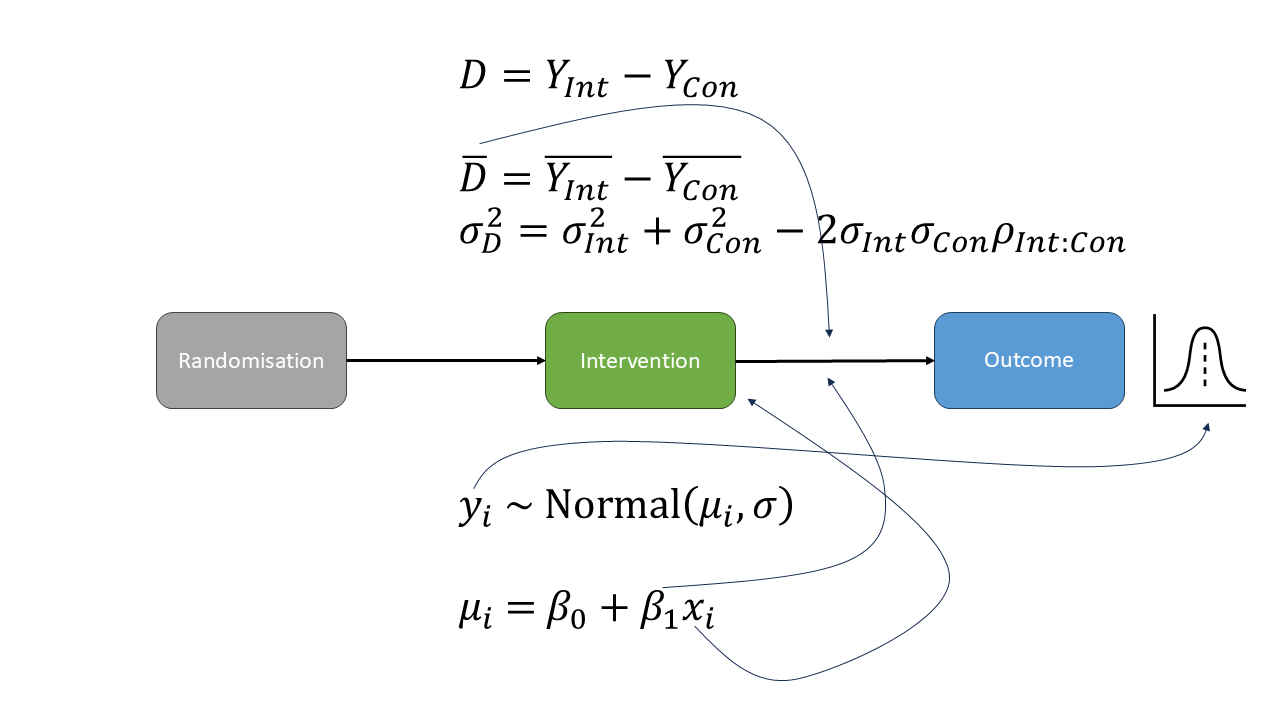
\includegraphics[width=\linewidth,height=8cm,keepaspectratio,alt={Estimand and estimate}]{images/Slide14.png}

}

\subcaption{\label{}Estimand and estimate}
\end{minipage}%
%
\begin{minipage}[t]{0.50\linewidth}

\raisebox{-\height}{

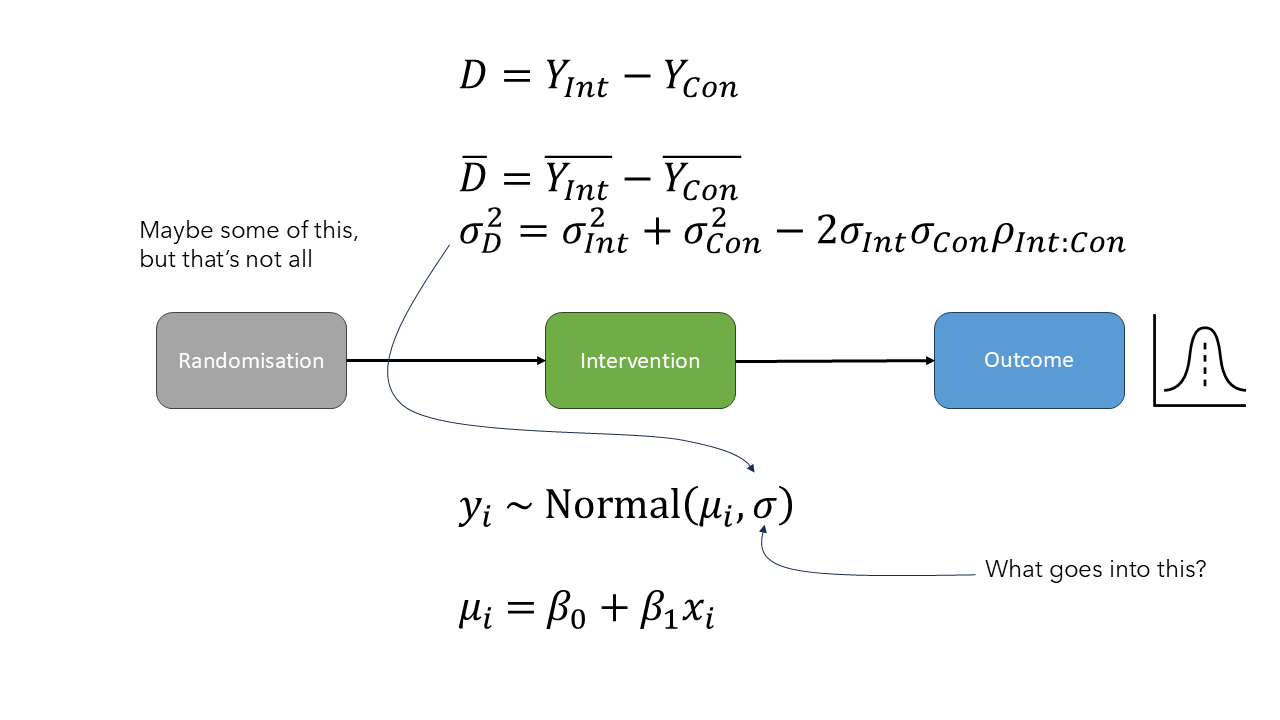
\includegraphics[width=\linewidth,height=8cm,keepaspectratio,alt={Variance in outcomes observed}]{images/Slide16.png}

}

\subcaption{\label{}Variance in outcomes observed}
\end{minipage}%
\newline
\begin{minipage}[t]{0.50\linewidth}

\raisebox{-\height}{

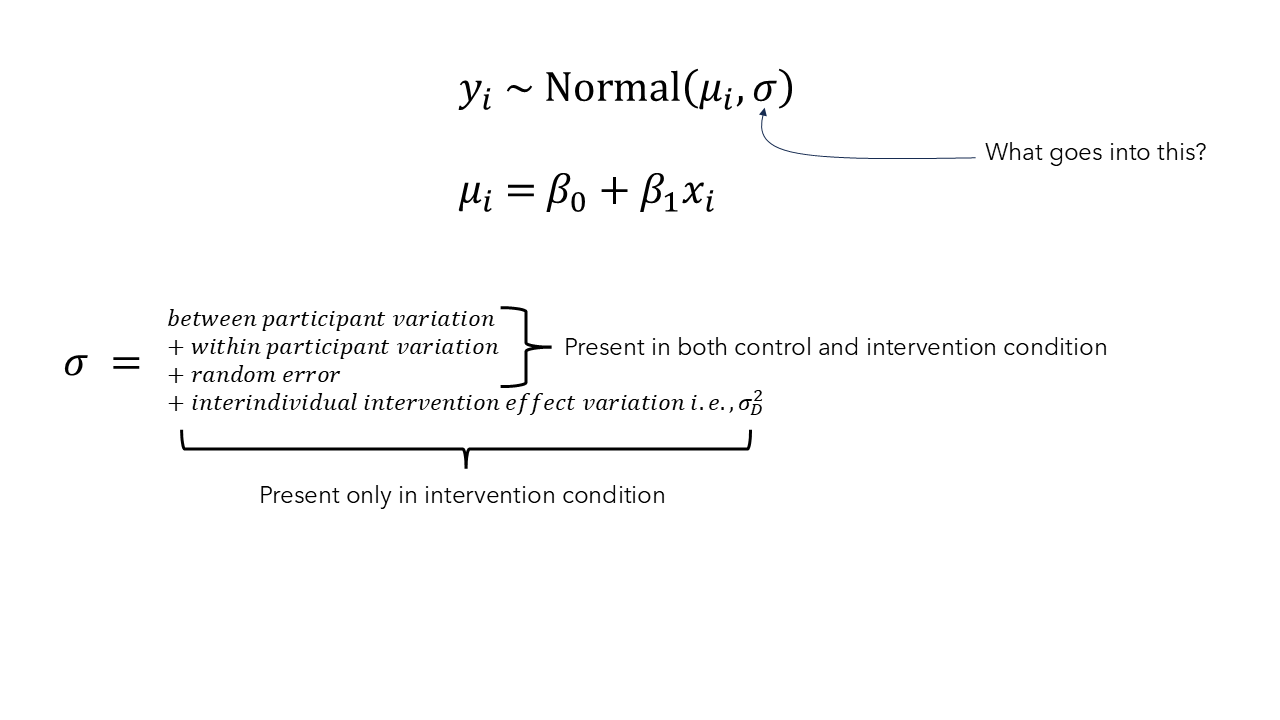
\includegraphics[width=\linewidth,height=8cm,keepaspectratio,alt={Sources of variance in outcomes observed}]{images/var_comp.png}

}

\subcaption{\label{}Sources of variance in outcomes observed}
\end{minipage}%
%
\begin{minipage}[t]{0.50\linewidth}

\raisebox{-\height}{

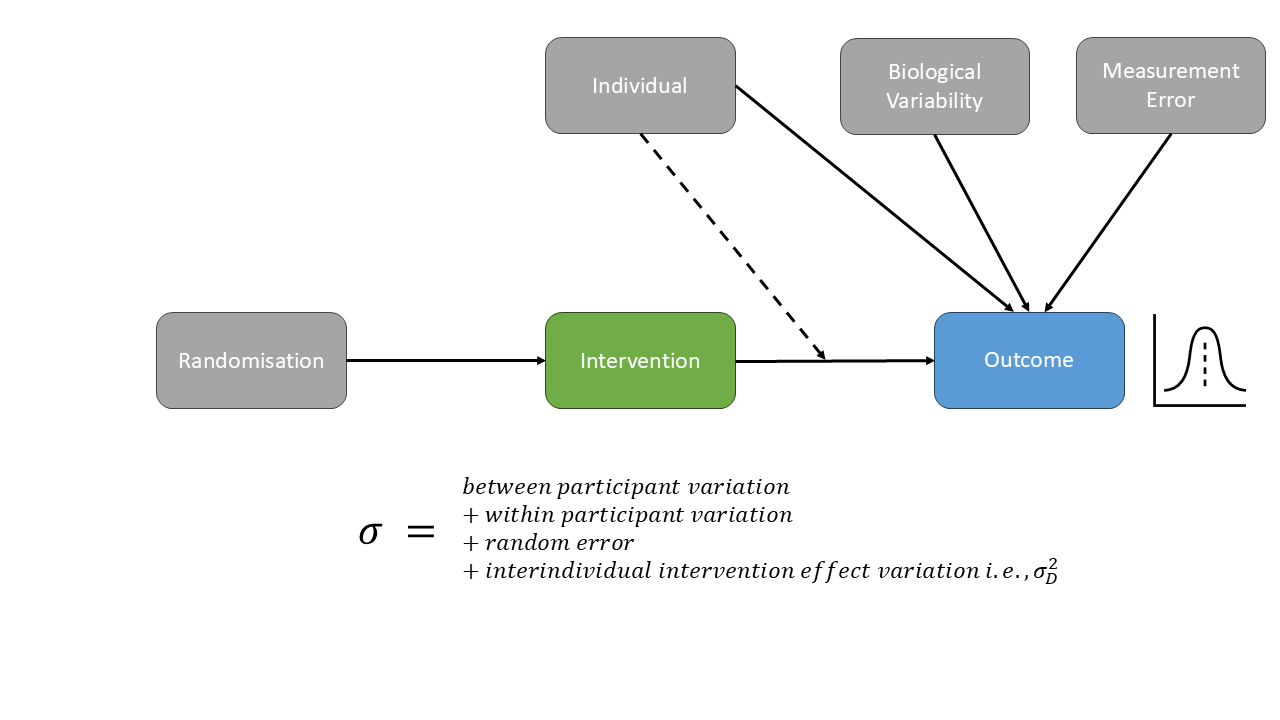
\includegraphics[width=\linewidth,height=8cm,keepaspectratio,alt={Sources of variance in outcomes observed}]{images/Slide29.png}

}

\subcaption{\label{}Sources of variance in outcomes observed}
\end{minipage}%

\caption{\label{fig-rct-logic}Mapping of estimand and estimate in the
randomised controlled trial design for estimating average intervention
effects alongside the directed acyclic graph. In (a) we have the defined
estimand of the average treatment effect, our estimate based on the
marginal distributions of interventions and controls (i.e., the causal
arrow from intervention to outcome), and the standard deviation of
treatment effects in addition to the general linear model estimator used
to yield and estimate of this average treatment effect. The components
of the general linear model are mapped to the their corresponding
components in the causal structure including the observed outcomes
\(y_i\), the randomly assigned intervention \(x_i\), and the estimated
average causal effect of the intervention compared to the control
\(\beta_1\). In (b), (c), and (d) it shows that some of the variance in
observed outcomes i.e., \(\sigma\), may be due to intervention effect
heterogeneity i.e., \(\sigma_{D}^2\) (the dashed arrow in (d) depicting
interaction of the individual with the intervention), but that there are
numerous other sources of variance and that these also differ between
the intervention and control conditions.}

\end{figure}%

The question of whether an intervention has introduced variation, that
is to say that there is some variation in the intervention effect and
not merely a fixed effect amongst participants, is essentially a
question of comparing variances in this type of study design i.e., an
RCT. In the context of an RCT with an inert control the variance
\(\sigma\) in observed outcomes \(y_i\) is due to between participant
variation, within participant variation, and other sources of random
error in the inert control condition, whereas in the intervention
condition only will there potentially be the additional source of
variation that is the interindividual variation of the intervention
effect itself (i.e., \(\sigma_{D}^2\)).

For RCTs it is a simple extension of the traditional general linear
model to a so-called location-scale model in which variances are
modelled directly, for example including the condition as a predictor in
the model for this parameter:

\begin{equation}\protect\phantomsection\label{eq-location-scale}{
\begin{aligned}
y_i &\sim \text{Normal}(\mu_i, \sigma_i) \\
\mu_i &= \beta_0 + \beta_1 x_i \\
\sigma_i &= \alpha_0 + \alpha_1 x_i
\end{aligned}
}\end{equation}

where now \(\alpha_0\) reflects the variance in the control condition
and \(\alpha_1\) estimates the effect of the intervention on the
variance.

There are also various effect size statistics that can be calculated for
the comparison of variances such as the standard deviation of individual
responses (\(SD_{IR}\)) (Atkinson \& Batterham, 2015; Hopkins, 2015),
the log ratio of standard deviations (\(\text{ln}VR\)) and the log
coefficient of variation ratio (\(\text{ln}CVR\)) (Nakagawa et al.,
2015; Senior et al., 2020), as well as various other statistical tests
for the comparison of variances (Mills et al., 2021). These effect size
statistics are particularly useful in the context of meta-analytic
approaches for examining the presence (or not) of interindividual
intervention effect heterogeneity. However, these effects sizes do come
with inherent assumptions that need to be considered when drawing
inferences about effect heterogeneity in randomised trials. These
include strong assumptions about the correlation between potential
outcomes (i.e., the value of the unobservable \(\rho_{Int:Con}\)) as
well as assumptions about the relationship between means and variances
(i.e., the \(SD_{IR}\) and \(\text{ln}VR\) assume the relationship to be
zero, whilst the \(\text{ln}CVR\) assumes it to be proportional).

The fact that \(\rho_{Int:Con}\) is not directly observable has been
termed the fundamental problem of causal inference and is why in RCTs we
focus upon the average intervention effect as the estimand of interest
(because we can only observe a outcomes under a single condition per
individual participant and not their potential outcome in the unobserved
condition). Caldwell et al.~(2025) show that the assumed value of the
unobservable \(\rho_{Int:Con}\) in fact depends on the ratio between the
observed standard deviations in the intervention and control conditions
(see https://osf.io/d59ru/files/7f6sq).

The mean-variance relationship also is ubiquitous in most natural
systems, and certainly in outcomes typical of resistance training
studies (Nuzzo et al., 2024; Steele et al., 2023), largely due to errors
being multiplicative i.e., increase as the mean increases. As such,
given that in the context of a RCT of a resistance training intervention
compared to an inert control we typically expect an increase in the mean
of outcomes such as strength or hypertrophy (assuming the intervention
is on average effective), any variance comparisons should account for
this possible impact in order to differentiate this coupling of the
parameters from the introduction of variance due to the intervention
\emph{qua} intervention. For a single trial, either the location-scale
model or use of the \(\text{ln}CVR\) is thus preferable.

A further issue is that the typical RCT in resistance training is
woefully underpowered to detect what could be considered realistic
variance ratios that we may want to detect between controls and
interventions. For example, in their simulations Caldwell et al.~(2025)
show that the typical study of n=20-30 participants may have
\textless25\% power to detect these differences and thus the
introduction of additional variance by the intervention. Thus,
meta-analytic approaches are incredibly value for exploring this
question, and with meta-analytic approaches we are also able to go one
step farther and directly model the ratio of variances between
interventions and controls whilst adjusting for the mean outcomes.

Considering the causal logic of the RCT, and the assumptions that need
to be examined when making variance comparisons for the purpose of
inference regarding intervention effect heterogeneity, in this paper I
re-examine the question of whether there is meaningful resistance
training intervention effect heterogeneity. To do so I take a
meta-analytic approach and use the large scale dataset of RCTs examining
resistance training interventions compared with inert controls that we
have previously presented (Steele et al., 2023).

\section{Methods}\label{methods}

All data, code, and materials for the present work are available at: ADD
LINKS. All packages used for analysis are cited in the corresponding
report generated by the grateful package.

\subsection{Dataset}\label{dataset}

In Steele et al.~(2023) we utilised the studies previously
systematically reviewed by Polito et al.~(2021) which were all RCTs of
resistance training interventions compared to non-training controls
where it could be expected that the control conditions were essentially
inert. We re-extracted data from the studies they identified and full
details of this dataset can be seen in Steele et al.~(2023) in addition
to the data being openly available (INSERT LINKS). Here I limit the
dataset to only studies of untrained participants (see footnote 1) and
explore the both the pooled strength and pooled hypertrophy outcomes.

\subsection{Analysis}\label{analysis}

An arm-based approach was taken using a multilevel meta-analytic model
of the log transformed standard deviations for each outcome at
post-intervention regressed upon the log transformed means for each
outcome at post-intervention and the arm from which these variances came
(i.e., intervention or control) allowing for comparison of variances
between arms whilst adjusting for the population mean-variance
relationship. The model was thus:

\begin{equation}\protect\phantomsection\label{eq-mean-var-meta}{
\begin{aligned}
\text{ln}(\hat{\sigma}_{ijk})=\beta_{0}+\tau_{1i}+\tau_{2j}+\tau_{3k}+\beta_{1}\text{ln}(\hat{\mu}_{ijk})+\beta_{2} x_{Cond}+\epsilon_{ijk}+m_{ijk}
\end{aligned}
}\end{equation}

where \(\text{ln}(\hat{\sigma}_{ijk}))\) is the log transformed standard
deviation of outcomes for the \(k^{th}\) outcome in the \(j^{th}\) arm
in the \(i^{th}\) study, \(\text{ln}(\hat{\mu}_{ijk}))\) is the log
transformed mean of outcomes with the same subscripts, \(\beta_{0}\) is
the average log transformed standard deviation in the control arms,
\(\beta_{1}\) is the slope of the log transformed mean upon the log
transformed standard deviation, \(\tau_{1i}\), \(\tau_{2j}\), and
\(\tau_{3k}\) are the respective normally distributed variances for
study, arm, and effect, \(\epsilon_{ijk}\) and \(m_{ijk}\) are similarly
the residual variance and sampling errors respectively, finally
\(x_{Cond}\) is a categorical predictor indicating whether and effect is
from a control or intervention arm and \(|beta_{2}\) reflects the
estimate of the average difference in variances between the control and
intervention arms.

As noted variance comparisons in RCTs inherently make assumptions
regarding the unobservable correlation between potential outcomes
(\(\rho_{Int:Con}\)). As such, in order to draw justifiable conclusions
from the analysis I perform here we should check these assumptions. I
calculate this for all the included variance contrasts in the
meta-analytic dataset and examine whether the empirical distribution of
assumed values are a justifiable assumption to allow us to treat our
variance comparisons as indicative of whether there is, or is not, any
interindividual intervention effect heterogeneity (see
https://osf.io/cg63r).

To do so I examine with the same dataset the meta-analytic estimate for
\(\rho_{Pre:Post}\) in both intervention and control groups. Typically
using the marginal estimate
\(\overline{D}=\overline{Y_{Post}}-\overline{Y_{Pre}}\) is not an
unbiased estimated of \(D=Y_{Int}-Y_{Con}\) and can be misleading
regarding the presence, or not, of interindividual intervention effect
heterogeneity\^{}2. However, in the case of resistance training
interventions in healthy participants with strength/hypertrophy outcomes
it is in fact a relatively unbiased estimate of \(D\)\^{}3. As such,
\(\rho_{Pre:Post}\) might be a reasonable estimate of \(\rho_{Int:Con}\)
and so I compare this with the calculated values of assumed
\(\rho_{Int:Con}\).

\section{Results}\label{results}

and the meta-analytically estimated (using a similar multilevel model
structure as noted above) values of \(\rho_{Pre:Post}\) are in line with
the values of \(\rho_{Pre:Post}\) (Strength Outcomes: Intervention
groups ρ\_(Pre:Post)=0.500 {[}95\%CI:0.365, 0.614{]}, Control groups
ρ\_(Pre:Post)=0.867 {[}95\%CI:0.705, 0.943{]}; Hypertrophy Outcomes:
Intervention groups ρ\_(Pre:Post)=0.827 {[}95\%CI:0.762, 0.875{]},
Control groups ρ\_(Pre:Post)=0.965 {[}95\%CI:0.900, 0.988{]}).




\end{document}
